\documentclass[varwidth=true, border=2pt]{standalone}

\usepackage{pgfplots}
\usepackage{tikz}
\usetikzlibrary{patterns}

\begin{document}
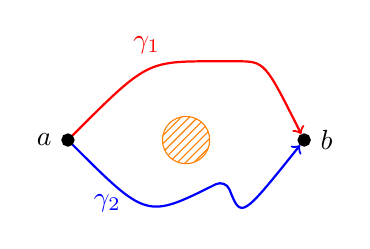
\begin{tikzpicture}
    \tikzstyle{point}=[circle,thick,draw=black,fill=black,inner sep=0pt,minimum width=4pt,minimum height=4pt]
    \node (a)[point,label=180:$a$] at (0,0) {};
    \node (b)[point,label=0:$b$]   at (3, 0) {};
    \draw[orange,pattern color=orange,pattern=north east lines] (1.5,0) circle (0.3cm);
    \draw [rounded corners,->, thick, red] (a) .. controls (1,1) .. (2,1) .. controls (2.5,1) .. (b);
    \draw [rounded corners,->, thick, blue] (a) .. controls (1,-1) .. (2,-0.5) .. controls (2.2,-1) .. (b);
    \node at (1,1.2) [red] {$\gamma_1$};
    \node at (0.5,-0.8) [blue] {$\gamma_2$};
\end{tikzpicture}
\end{document}
